\section{Introduction}
A long-term goal of robotics research is the introduction of intelligent household robots.
Such robots would face complex tasks, such as setting
dinner tables and doing laundry. Planning for these long-horizon tasks is infeasible
using only motion planning due to the sheer number of steps involved, making apparent the need
for a hierarchical system of reasoning.

Recent methods for hierarchical planning focus on the intersection of high level \emph{task} planning
and low level \emph{motion} planning~\cite{srivastava2014combined, kaelbling2011hierarchical,
lagriffoul2014orientation}. In this framework, the (classical) task planner produces
a symbolic plan containing a sequence of actions to reach a goal
state, and heuristic sampling techniques propose concrete values for
the continuous variables in the plan, thus grounding it. This process of assigning
candidate values to the plan variables is known as \emph{plan refinement}. These candidate values
are then checked locally for feasibility by calling a motion planner.

This hierarchy enforces abstraction between the role of the task planner and that of the motion planner:
the task planner maintains no knowledge of the environment geometry, and the
motion planner has no understanding of the overall goal.
A central challenge in building such a system is designing good heuristics for the sampling in plan refinement.

\begin{figure}[h]
  \centering
    \noindent
    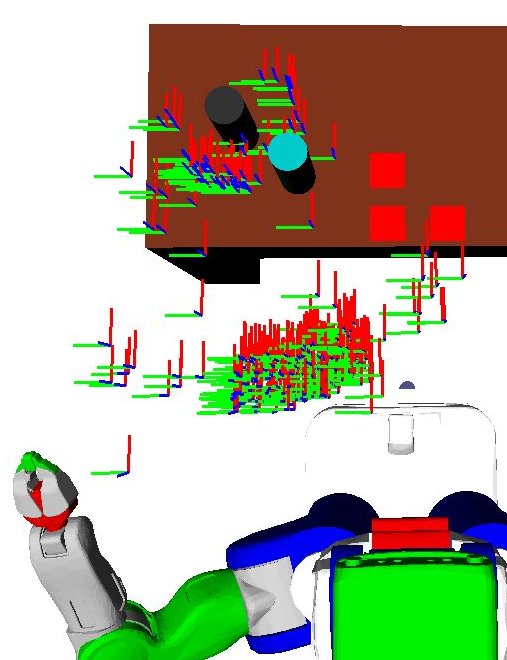
\includegraphics[scale=0.2]{images/move_grasp.png}\hspace{10 mm}
    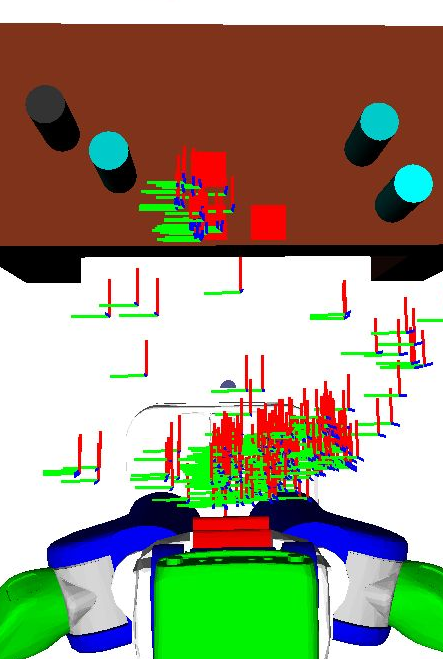
\includegraphics[scale=0.2]{images/move_putdown.png}
  \caption{Screenshots showing some distributions learned by our system in one experimental
    setup. The robot is tasked with grasping the black cylinder and putting it down on the
    central red square. The left image shows learned base motion and grasping distributions,
    and the right shows learned base motion and putdown distributions. The grasp distribution
    properly learned to avoid the region close to the blue obstruction. We sample from these distributions
    to refine the high level plan, rather than relying on hand-coded ones.}
  \label{fig:cover}
\end{figure}

Our work improves directly upon the task and motion planning system
presented by Srivastava et al.~\cite{srivastava2014combined}. They propose
an \emph{interface layer} for plan refinement, which performs an exhaustive
backtracking search over a discrete set of parameter values for refining
the symbolic plan into a set of collision-free trajectories. If a motion
planning feasible refinement is not found within the resource limit,
symbolic error information is propagated back to the task planner, and a new symbolic plan is produced.
The system uses an off-the-shelf classical task planner and motion planner, both as black boxes.
We build upon this framework because it is easy to separate the plan refinement module from the task planning module.

A key limitation of task and motion planning systems is that they typically rely on hand-coded heuristic
sampling distributions for plan refinement. These distributions are tuned for the specific
geometric properties of the environment and its objects.
This restriction has several negative implications: the parameters of the
hand-coded distributions must be fine-tuned when running the system in a new setting, and the
resulting refinement distributions lack robustness.

In this work, we apply reinforcement learning to find good proposal distributions
for symbolic plan refinement. We take inspiration
from the work of Zhang and Dietterich~\cite{JobShopSched}, who applied reinforcement learning
to planning problems in a job shop scheduling setting. Using methods adapted from
Zucker et al.~\cite{workspacebias}, who train a configuration space sampler for motion planning
using features of the discretized workspace, we train a policy that
determines how to sample values for plan symbols, using policy optimization with linear function
approximation. Our approach allows the learned distributions to be continuous, robust to changes in
the environment, and trainable for any experimental setting, eliminating the need for hand-tuned
distribution parameters.

The three contributions of our work are as follows:
\begin{tightlist}
\item[1)] We present randomized refinement,
a novel local search algorithm for plan refinement. Randomized refinement maintains at
all times a set of values for all symbolic plan variables, then at each iteration randomly
resamples one whose current instantiation is causing a failure. This naturally guides
plan variable resampling intelligently and easily lends itself to reinforcement learning.
\item[2)] We describe how to formulate plan refinement (using randomized
refinement) in the standard reinforcement learning framework, so that sampling
distributions for plan variables can be learned instead of hand-coded. Our formulation optimizes for
minimizing the number of calls to the motion planner.
\item[3)] We present experiments to evaluate our approach
in a variety of test environments involving complicated grasp and putdown
actions with obstructions and base motion. Our experimental results demonstrate
comparable to improved performance for both motion planning time and number of calls to
the motion planner, when compared to the hand-coded distributions used in the original system.
\end{tightlist}